\documentclass[a4paper,11pt]{scrartcl}

\usepackage{ngerman}
\usepackage[utf8]{inputenc}

\usepackage{amsmath}
\usepackage{amsthm}
\usepackage{amsfonts}
\usepackage{amssymb}
\usepackage{amsbsy}


\usepackage{tensor}

\usepackage{tikz}

\usepackage{hyperref}
\renewcaptionname{ngerman}{\figurename}{Abb.}
\newcaptionname{ngerman}{\figureautorefname}{Abb.}

%Bezeichner
\newcommand{\U}{u} %Komponenten des Geschwindigkeitfeldes
\newcommand{\Ub}{\mathbf{\U}} %Geschwindigkeitsfeld
\newcommand{\tU}{\tilde{u}} %Komponenten des Geschwindigkeitfeldes
\newcommand{\tUb}{\mathbf{\tU}} %Geschwindigkeitsfeld
\newcommand{\V}{v} %Komponenten des Geschwindigkeitfeldes
\newcommand{\Vb}{\mathbf{\V}} %Geschwindigkeitsfeld
\renewcommand{\P}{p} %Druck
\newcommand{\g}{\mathbf{g}} % metrischer Tensor, Oberflaechenidentitaet
\newcommand{\lc}{\mathbf{E}} % Levi-Civita-Tensor
\newcommand{\gauss}{\mathcal{K}} % Gauss-Kruemmung
\newcommand{\ekin}{\textup{E}_{\textup{Kin}}} %kinetische Energie
\newcommand{\dtekin}{\dot{\textup{E}}_{\textup{Kin}}} %kinetische Energie
\newcommand{\landau}{\mathcal{O}}

% General
\newcommand{\vect}[1]{\mathbf{#1}}


%Raeume
\newcommand{\surf}{\mathcal{S}} %Oberflaeche
\newcommand{\uspace}{\mathcal{T}^{(1)}(\surf)} % Typ 1 Tensor; Co- bzw. Contravarintes Tangentialbuendel
\newcommand{\Tangent}{\mathsf{T}}
\newcommand{\R}{\mathbb{R}}

%Operatoren
\renewcommand{\div}{\operatorname{div}} %Divergenzoperator
\newcommand{\rot}{\operatorname{rot}} %Rotationsoperator
\newcommand{\lie}{\mathcal{L}} %Lie-Ableitung
\newcommand{\exd}{\mathbf{d}} %Aeussere Ableitung
\newcommand{\lrr}{\Delta^{\textup{Rr}}} %Rot-rot-Laplace
\newcommand{\ldg}{\Delta^{\textup{dG}}} %div-Grad-Laplace
\newcommand{\lgd}{\Delta^{\textup{Gd}}} %Grad-div-Laplace
\newcommand{\ldr}{\Delta^{\textup{DR}}} %Laplace-deRham
\newcommand{\jup}{\textup{j}} % teilweises inneres Produkt

% DEC declarations
\newcommand{\SC}{\mathcal{K}} % simplicial complex
\newcommand{\Vs}{\mathcal{V}} % set of vertices
\newcommand{\Es}{\mathcal{E}} % set of edges
\newcommand{\Fs}{\mathcal{T}} % set of faces
\newcommand{\face}{T} % one face
\newcommand{\FormSpace}{\Lambda^{1}} % space of 1 forms
\newcommand{\flatgb}[2]{\overset{#1 #2}{\g}}
\newcommand{\flatg}[2]{\overset{#1 #2}{g}}

\newcommand{\facesim}{\overset{\face}{\sim}}


%Zeug
\newcommand{\formComma}{\,\text{,}}
\newcommand{\formPeriod}{\,\text{.}}
\newcommand{\ingo}[1]{{\color{blue}#1}}



\title{Notizen zur DEC-Diskretisierung der Navier-Stokes-Gleichungen auf Oberflächen} 
\author{Ingo Nitschke}

\begin{document}
\maketitle
\tableofcontents

\section{Navier-Stokes-Gleichungen}

Es sei \( \Ub\in\uspace \) ein Geschwindigkeitsfeld auf der randlosen hinreichend glatten Oberfläche \( \surf \) mit contravarianten Komponenten
\( \U^{i} \) bzw. covarianten Komponenten \( \U_{i} = g_{ij}\U^{j} \), 
wobei \( g_{ij} \) die Komponenten des Metrischen Tensors \( \g \) sind.
Für ein inkompressibles homogenes Medium reduziert sich die Kontinuitätsgleichung zu 
\begin{align}\label{eq:konti}
  0 &= \div\Ub = *\exd*\Ub = \tensor{\U}{^{i}_{|i}} = \partial_{i}\U^{i} + \Gamma_{ij}^{i}\U^{j} \formPeriod
\end{align}
\( \Gamma_{ij}^{k} \) sind die Christoffelsymbole, welche die partiellen Ableitungen der Metrik beinhalten.
Der senkrechte Strich bezeichnet die covarianten Ableitungen.

Die kräftefreie Impulserhaltung in seiner differentiellen Form unter berücksichtigung der Kontinuitätsgleichung lautet \cite{deSimone2009}
\begin{align}\label{eq:impulsRaw}
   \dot{\Ub} + \nabla_{\Ub}\Ub &= \frac{1}{\rho}\div\mathbf{\sigma}\formComma
\end{align}
mit konstanter Dichte \( \rho \), Richtungsableitung \( \left[ \nabla_{\Ub}\Ub \right]_{i} = \U^{j}\U_{i|j} \)
und Oberflächenspannungtensor für inkompressible Fluide
\begin{align}
  \mathbf{\sigma} &= -\tilde{\P}\g + \mu\lie_{\Ub}\g\formPeriod
\end{align}
Dabei bezeichnet \( \mu = \rho\nu \) die dynamischen Viskosität, \( \nu \) die kinematische Viskosität,
\( \tilde{\P} \) den Druck und 
\begin{align}
  \left[ \lie_{\Ub}\g \right]_{ij} = \U_{i|j} + \U_{j|i} = \left[ \nabla\Ub + (\nabla\Ub)^{T} \right]_{ij}
\end{align}
die Lie-Ableitung des metrischen Tensors \( \g \) in Richtung \( \Ub \), welche somit zweimal den rate-of-deformation-Tensor quantifiziert \cite{marsden1983}.
Für die Divergenz des Spannungstensor \cite{deSimone2009} ergibt sich mit dem Rot-rot-Laplace \( \lrr = *\exd*\exd \) und Gaußscher-Krümmung \( \gauss \)
\begin{align}
  \div\mathbf{\sigma} &= \left\{ \tensor{\sigma}{_{i}^{j}_{|j}} \right\}
            = -\exd\tilde{\P} + \mu(\lrr\Ub + 2\gauss\Ub)
            = \left\{ -\partial_{i}\tilde{\P} + \mu\left( \tensor{\U}{_{i}^{|j}_{|j}} - \tensor{\U}{_{j|i}^{|j}} + 2\gauss\U_{i} \right) \right\} \formPeriod
\end{align}
Somit ergibt sich für \( \P := \rho^{-1}\tilde{\P} \) die Impulserhaltung \eqref{eq:impulsRaw} in seiner covarianten Form
\begin{align}
  \dot{\Ub} + \nabla_{\Ub}\Ub   - \nu\left( \lrr\Ub + 2\gauss\Ub \right) + \exd\P&= 0 \text{ bzw.} \label{eq:impuls}\\
  \dot{\U}_{i} + \U^{j}\U_{i|j} - \nu \left( \tensor{\U}{_{i}^{|j}_{|j}} - \tensor{\U}{_{j|i}^{|j}} + 2\gauss\U_{i}\right) + \partial_{i}\P &= 0 \formPeriod
\end{align}
Es sei hier darauf hingewiesen, dass wegen der Divergenzfreiheit von \( \Ub \) für den Laplace-deRham-Operator \( \ldr \)
\begin{align}
  -\ldr\Ub = *\exd*\exd\Ub + \exd*\exd*\Ub = *\exd*\exd\Ub = \lrr\Ub
\end{align}
gilt \cite{marsden1988} und somit (Weizenböck-Identität)
\begin{align}\label{eq:divfreeweizen}
  \lrr\Ub = \ldg\Ub - \gauss\Ub \formPeriod
\end{align}
\( \ldg\Ub = \left\{ \tensor{\U}{_{i}^{|j}_{|j}} \right\} \) ist der Div-Grad- bzw. (minus) Bochner-Laplace-Operator.

\subsection{Dissipation}
  Betrachten wir den Term \( 2\nu\gauss\Ub \) in \eqref{eq:impuls}, dann könnten wir geneigt sein diesen Term als Scheinkraft in Abhängigkeit der Krümmung zu interpretieren.
  Da \( \gauss \) alle möglichen positiven oder negativen Werte annehmen könnte, wollen wir nun kurz untersuchen, ob obige Navier-Stokes-Gleichungen dissipativ sind
  und die kinetische Energie des Gesamtsystems entgegen der Intuition nicht auch zunehmen könnte.
  D.h. wir zeigen, dass
  \begin{align}
    \dtekin = \frac{\textup{d}}{\textup{d}t} \frac{1}{2} \int_{\surf} \left\| \Ub \right\|^{2}\mu
                = \int_{\surf} \left\langle \Ub , \dot{\Ub} \right\rangle \mu
                \le 0
  \end{align}
  unter \eqref{eq:impuls} und \eqref{eq:konti} gilt.

  Für den Druckgradienten ergibt sich wegen der Divergenzfreiheit
  \begin{align}
    \int_{\surf} \left\langle \Ub , -\exd\P \right\rangle \mu
        &=  -\int_{\surf} \U^{i}\partial_{i}\P \mu
         = -\int_{\surf} \U^{i} \P_{|i} \mu
         =  \int_{\surf}  \tensor{\U}{^{i}_{|i}}\P \mu = 0 \formPeriod
  \end{align}
  Für die Advektion gilt
  \begin{align}
    \int_{\surf} \left\langle \Ub , -\nabla_{\Ub}\Ub \right\rangle \mu
        &=  -\int_{\surf} \U^{i}\U^{j}\U_{i|j} \mu
         = \int_{\surf} \left( \U^{i}\U^{j} \right)_{|j}\U_{i} \mu \\
        &= \int_{\surf} \U^{i}\left( \U_{i|j}\U^{j} + \U_{i}\tensor{\U}{^{j}_{|j}} \right)\mu
         = \int_{\surf} \U^{i}\U_{i|j}\U^{j}\mu \\
        &= \int_{\surf} \left\langle \Ub , \nabla_{\Ub}\Ub \right\rangle \mu
  \end{align}
  und folglich
  \begin{align}
    \int_{\surf} \left\langle \Ub , -\nabla_{\Ub}\Ub \right\rangle \mu = 0 \formPeriod
  \end{align}
  Somit ist gezeigt, dass für die Euler-Gleichungen, d.h. \( \nu=0 \), wie zu erwarten \( \dtekin = 0 \) gilt.
  Für viskose Fluide, d.h. \( \nu > 0 \), ergibt sich
  \begin{align}
    \int_{\surf} \left\langle \Ub , \nu\left( \lrr\Ub + 2\gauss\Ub\right) \right\rangle \mu
      &= \nu \int_{\surf} \left\langle \Ub , \div\lie_{\Ub}\g \right\rangle \mu 
       = \nu \int_{\surf} \U^{i} \tensor{\left[\lie_{\Ub}\g \right]}{_{ij}^{|j}} \mu\\
      &= -\nu \int_{\surf} \U^{i|j}\left( \U_{i|j} + \U_{j|i} \right) \mu\\
      &= -\nu \int_{\surf} \nabla\Ub : \left( \nabla\Ub + (\nabla\Ub)^{T} \right)\mu \\
      &\overset{(*)}{=} -\frac{\nu}{2} \int_{\surf} \left\| \nabla\Ub + (\nabla\Ub)^{T}  \right\|^{2} \mu\\
      &= -\frac{\nu}{2} \int_{\surf} \left\| \lie_{\Ub}\g  \right\|^{2} \mu < 0
      \formPeriod
  \end{align}
  \( (*) \) ergibt sich, weil im rechten Argument zweimal die Projektion in den Raum der symmetrischen Typ-2-Tensoren steht,
  ein symmetrischer idempotenter Operator.
  Wir können hier aber auch im speziellen nachrechnen
  \begin{align}
    \U^{i|j}\left( \U_{i|j} + \U_{j|i} \right)
      &= \frac{1}{2}\left( \U^{i|j} + \U^{j|i} + \U^{i|j} -  \U^{j|i}\right)\left( \U_{i|j} + \U_{j|i} \right) \\
      &= \frac{1}{2}\left[\left( \U^{i|j} + \U^{j|i} \right)\left( \U_{i|j} + \U_{j|i} \right)
          +\left(  \U^{i|j}\U_{i|j} - \U^{j|i}\U_{j|i} \right)
          +\left(  \U^{i|j}\U_{j|i} -  \U^{j|i}\U_{i|j}\right)\right] \\
      &= \frac{1}{2}\left( \U^{i|j} + \U^{j|i} \right)\left( \U_{i|j} + \U_{j|i} \right) \formPeriod
  \end{align}
  Schlußendlich können wir \( \dtekin \le 0 \) folgern für \( \nu \ge 0 \).
  Wir beobachten außerdem, dass das System genau dann nicht dissipativ ist,
  wenn das Fluid nicht viskos oder die Strömung \(\Ub  \) ein Killing-Vektor-Feld ist,
  d.h.
  \begin{align}
    \dtekin = 0 \quad\Longleftrightarrow\quad \nu = 0 \quad \vee \quad \lie_{\Ub}\g = 0 \formPeriod
  \end{align}
  Letztere Bedingung bringt uns eine interessante Erkenntnis. 
  Bei roationssymmetrischen Oberflächen, wobei \( \phi \) die lokale Rotationskoordinate sein soll,
  d.h. \( \partial_{\phi}\g = 0 \), ist die Lösung \( \Ub = \partial_{\phi} \) nicht dissipativ.
  
\section{Linearisierung der Advektion}

  Für eine bessere Handhabe des Advektionstermes, linearisieren wir diesen mittels Taylorapproximation an einem bekannten Geschwindigkeitsfeld \( \tUb \) und dessen Gradienten 
  \( \nabla\tUb \), d.h. in der covarianten Form ergibt sich
  \begin{align}
     \left[ \nabla_{\Ub}\Ub  \right]_{i} &= \U^{j}\U_{i|j}\\
         &\approx \tU^{j}\tU_{i|j} + \tU_{i|j}\left( \U^{j} - \tU^{j} \right) + \tU^{j}\left( \U_{i|j} - \tU_{i|j} \right) \\
         &= \U^{j}\tU_{i|j} + \tU^{j}\U_{i|j} - \tU^{j}\tU_{i|j} \\
         &= \left[ \nabla_{\tUb}\Ub + \nabla_{\Ub}\tUb - \nabla_{\tUb}\tUb\right]_{i}\formPeriod \label{eq:Lin1}
  \end{align}
  Mit Hilfe des Levi-Cevita-Tensors \( \lc \) (definiert über die Volumenform durch \( \lc(\Ub,\Vb) = \mu(\Ub,\Vb) \)) erhalten wir die Identität
  \begin{align}
    \left( \rot\Ub \right)\left[ *\Vb \right]_{i}
      &= E_{il}E_{jk}\V^{l}\U^{j|k} 
       = \left( g_{ij}g_{lk} - g_{ik}g_{lj} \right)\V^{l}\U^{j|k}
       = \V^{l}\left( \U_{i|l} - \U_{l|i} \right) \\
      &= \left[ \nabla_{\Vb}\Ub \right]_{i} - \left[ \Vb\cdot\nabla\Ub \right]_{i}
  \end{align}
  für \( \Ub,\Vb\in\uspace \).
  Desweiteren gilt
  \begin{align}
    \left[ \Vb\cdot\nabla\Ub + \Ub\cdot\nabla\Vb\right]_{i}
        &= \V^{l}\U_{l|i} + \U_{l}\tensor{\V}{^{l}_{|i}}
         = \left( \V^{l}\U_{l} \right)_{|i} 
         = \partial_{i}\left\langle \Vb, \Ub \right\rangle
  \end{align}
  und im Speziellem 
  \begin{align}
    2\left[ \Ub\cdot\nabla\Ub \right] = \partial_{i}\left\| \Ub \right\|^{2} \formPeriod
  \end{align}
  Setzen wir diese drei Gleichungen und \( \rot\tUb = -\div(*\tUb) \) in die Linearisierung \eqref{eq:Lin1} ein, dann erhalten wir
  \begin{align}\label{eq:Lin2}
    \nabla_{\Ub}\Ub &\approx \exd\left( \left\langle \Ub, \tUb \right\rangle - \frac{1}{2}\left\| \tUb \right\|^{2} \right)
                            +\left( \rot\Ub - \rot\tUb \right)(*\tUb)
                            -\div(*\tUb)(*\Ub) \formPeriod
  \end{align}

\section{Diskretisierung}
\subsection{Zeitdiskrete Gleichungen}
  Wir nutzen ein semi-implizites Eulerschema für die Zeitdiskretisierung, 
  wobei der Advektionsterm zur Zeit \( t_{k+1} \) mit der Lösung \( \Ub_{k} \) zur Zeit \( t_{k} \) gemäß \eqref{eq:Lin2} linearisiert wird.
  Somit ist für \( \tau_{k} := t_{k+1} - t_{k} \) und der Startlösung \( \Ub_{0} \) eine Folge von linearen Differentialgleichungssystemen zu lösen,
  d.h. für \( k=0,1,2,\ldots \) finde \( \Ub_{k+1}\in C^{2}\left(\surf, \uspace\right) \) und \( q_{k+1},p_{k+1}\in C^{1}(\surf) \), so dass
  \begin{align}
    \frac{1}{\tau_{k}}\Ub_{k+1} - \nu\left( \lrr\Ub_{k+1} + 2\gauss\Ub_{k+1} \right) + \exd q_{k+1}
        &+ (*\Ub_{k})\rot\Ub_{k+1} - \div(*\Ub_{k})(*\Ub_{k+1}) \notag\\
              &= \frac{1}{\tau_{k}}\Ub_{k} + (*\Ub_{k})\rot\Ub_{k} \label{eq:NS1DisTime}\\
    \left\langle \Ub_{k}, \Ub_{k+1} \right\rangle + \P_{k+1} - q_{k+1} 
          &= \frac{1}{2}\left\| \Ub_{k} \right\|^{2} \label{eq:NS3DisTime}\\
    \div\Ub_{k+1} &= 0
  \end{align}
  auf \( \surf \) gilt.

\subsection{DEC-Diskretisierung}
  Für eine Einführung in das Diskrete Äußere Kalkül (DEC) siehe \cite{Desbrun2005, Hirani2003, DiplomIngo2014}.
  Die DEC-Notationen sind weitgehend konsistent zu \cite{Nestler2016}.

  \subsubsection{Zusätzliche Definitionen und Notationen}
    \paragraph{Zusammenhangsrelation \( \sim \) von Kanten}
      Wir nennen zwei Kanten \( e,\tilde{e}\in\Es \) zusammenhängend, wenn sie sich einen Knoten teilen und schreiben
      \begin{align}
        \tilde{e} \sim e \quad :\Longleftrightarrow\quad
          \exists!v\in\Vs:\, v\prec\tilde{e} \wedge v\prec e \formPeriod
      \end{align}
      Zwei solche Kanten sind in \autoref{fig:oneVertexTwoEdges} dargestellt.
      Existiert zusätzlich ein Dreieck \( \face\succ e \) für das auch \( \tilde{e}\prec\face \) gilt, 
      dann schreiben wir \( e \facesim \tilde{e} \).

    \paragraph{Diskrete Metrik}
      Zwei linear unabhängige  Vektoren \( \vect{e},\tilde{\vect{e}}\in V_{\vect{e}\tilde{\vect{e}}} := \operatorname{Span}\left\{  \vect{e},\tilde{\vect{e}} \right\} \)       
      bilden eine konstante (flache) Metrik \( \flatgb{\vect{e}}{\tilde{\vect{e}}}\in(\Tangent^{*}V_{\vect{e}\tilde{\vect{e}}})^{2} \).
      Diese beiden Vektoren können zum Beispiel Kanten darstellen, wie in \autoref{fig:oneVertexTwoEdges},
      dann schreiben wir auch \( \flatgb{e}{\tilde{e}} \), vgl. hierzu auch \cite{Nestler2016}.
      Da Vektoren (mit Fußpunkt) gerade die Ableitung ihrer eigenen baryzentrischen Parametrisierung sind, 
      ergibt sich die Metrik auf natürlicher Art durch
      \begin{align}
        \flatgb{\vect{e}}{\tilde{\vect{e}}}
            &=
                \begin{bmatrix}
                  \flatg{\vect{e}}{\tilde{\vect{e}}}_{\vect{e}\vect{e}} & \flatg{\vect{e}}{\tilde{\vect{e}}}_{\vect{e}\tilde{\vect{e}}} \\
                  \flatg{\vect{e}}{\tilde{\vect{e}}}_{\vect{e}\tilde{\vect{e}}} & \flatg{\tilde{\vect{e}}}{\tilde{\vect{e}}}_{\vect{e}\tilde{\vect{e}}}
                \end{bmatrix}
             = s_{\vect{e}\tilde{\vect{e}}} 
                  \begin{bmatrix}
                    \left\| \vect{e} \right\|^{2} & \vect{e}\cdot\tilde{\vect{e}} \\
                    \vect{e}\cdot\tilde{\vect{e}} & \left\| \tilde{\vect{e}} \right\|^{2}
                  \end{bmatrix} \formPeriod
      \end{align}
      Das Vorzeichen \( s_{\vect{e}\tilde{\vect{e}}} \in \left\{ -1, +1 \right\} \) ist der Erhaltung der Orientierung der zugrunde liegenden Oberfläche geschuldet
      und definiert sich über
      \begin{align}
        s_{\vect{e}\tilde{\vect{e}}}
          &:=
              \begin{cases}
                +1 & \text{if }\measuredangle(\vect{e},\tilde{\vect{e}}) < \pi \\
                -1 & \text{if }\measuredangle(\vect{e},\tilde{\vect{e}}) > \pi
              \end{cases}\formPeriod
      \end{align}
      Der Fall \( \measuredangle(\vect{e},\tilde{\vect{e}}) = \pi \) kann wegen der Forderung nach linearer Unabhängigkeit nicht eintreten.
      Für Kanten \( e\sim\tilde{e} \) ist \( s_{e,\tilde{e}} \) auch eindeutig durch die Struktur des Kantenskeletts bestimmt.
      In \autoref{fig:correctEdgeOrientation} sind die Kanten so um \( e \) orientiert, dass \( s_{e,\cdot} \) immer positiv ist und somit jede umorientierung einer Kante ein
      Vorzeichenwechsel der Metrik zu Folge hat.

      Der Betrag des Volumenelementes ergibt sich nun durch
      \begin{align}
        \sqrt{\left| \flatgb{\vect{e}}{\tilde{\vect{e}}} \right|}
            &= \sqrt{\left\| \vect{e} \right\|^{2}\left\| \tilde{\vect{e}} \right\|^{2} 
                        - \left( \vect{e}\cdot\tilde{\vect{e}}\right)^{2}} \formComma
      \end{align}
      und die inverse Metrik durch
      \begin{align}
        \flatgb{\vect{e}}{\tilde{\vect{e}}}^{-1}
            &=
                \begin{bmatrix}
                  \flatg{\vect{e}}{\tilde{\vect{e}}}^{\vect{e}\vect{e}} & \flatg{\vect{e}}{\tilde{\vect{e}}}^{\vect{e}\tilde{\vect{e}}} \\
                  \flatg{\vect{e}}{\tilde{\vect{e}}}^{\vect{e}\tilde{\vect{e}}} & \flatg{\tilde{\vect{e}}}{\tilde{\vect{e}}}^{\vect{e}\tilde{\vect{e}}}
                \end{bmatrix}
             = 
                \frac{s_{\vect{e}\tilde{\vect{e}}}}{\left| \flatgb{\vect{e}}{\tilde{\vect{e}}} \right|}
                  \begin{bmatrix}
                   \left\| \tilde{\vect{e}} \right\|^{2} & -\vect{e}\cdot\tilde{\vect{e}} \\
                    -\vect{e}\cdot\tilde{\vect{e}} & \left\| \vect{e} \right\|^{2}                   
                  \end{bmatrix} \formPeriod
      \end{align}

      Der Vorteil, dieser diskreten Metrik ist, dass mit \autoref{sec:approxOneForm} wir eine Erweiterung einer 1-Form der Oberfläche als Taylor-Approximation an einer Kante formulieren
      können. Die diskrete Metrik selbst ist auch eine konstante Approximation einer erweiterten Metrik, welche von der Oberfläche kommt.
      Somit können wir Terme die den Metrischen Tensor, aber nicht dessen Ableitungen, in der diskreten abstrakten 1-Form (definiert auf der abstrakten Kante \( \pi(e) \))
      mit der konstanten diskreten Metrik konsistent approximieren und diese vor das Integral schreiben.
      Dieses Vorgehen erweitert das diskrete Kalkül so, dass wir nun in gewohnter Weise mit diskreten 1-Formen rechnen können, wie im kontinuierlichen Fall, sofern wir nicht ableiten.
      Zum Beispiel können wir für \( \alpha = \alpha_{1}d\lambda^{1} + \alpha_{2}d\lambda^{2} \) mit \( \lambda^{1} \) und \( \lambda^{2} \) die
      barycentrischen Koordinaten der abstrakten Kante \( \pi(e) \) und \( \pi(\tilde{e}) \), folgendes konsistent für \( h\rightarrow 0 \) approximieren
      \begin{align}
        \left( *\alpha \right)_{h}(e)
            &= \left( \frac{1}{\sqrt{|\g|}}\left[ \left( g_{12}\alpha_{1} - g_{11}\alpha_{2} \right)d\lambda^{1} 
                                          +\left( g_{22}\alpha_{1} - g_{12}\alpha_{2} \right)d\lambda^{2}\right] \right)_{h}(e) \\
            &\approx \frac{1}{\sqrt{\left| \flatgb{\vect{e}}{\tilde{\vect{e}}} \right|}}
                \left[ \flatg{\vect{e}}{\tilde{\vect{e}}}_{\vect{e}\tilde{\vect{e}}}\left( \alpha_{1}d\lambda^{1} \right)_{h}(e) 
                      -\flatg{\vect{e}}{\tilde{\vect{e}}}_{\vect{e}\vect{e}}\left( \alpha_{2}d\lambda^{1} \right)_{h}(e) \right] \\
            &\approx \frac{1}{\sqrt{\left| \flatgb{\vect{e}}{\tilde{\vect{e}}} \right|}}
                \left[ \flatg{\vect{e}}{\tilde{\vect{e}}}_{\vect{e}\tilde{\vect{e}}}\left( \alpha \right)_{h}(e) 
                      -\flatg{\vect{e}}{\tilde{\vect{e}}}_{\vect{e}\vect{e}}\left( \alpha \right)_{h}(\tilde{e}) \right] \formPeriod\label{eq:hodgeApproxTwoEdges}
      \end{align}
      Letztere konsistente Approximation folgt aus der konstanten Interpolation auf den Kanten an der gemeinsamen Ecke \( v\prec e , \tilde{e}\ \).

      \ingo{Hier muss noch so einiges an Formalismus und sauberen Konsistenzbeweisen getan werden. Dann haben wir aber eine großartige Erweiterung zum klassischen diskreten Kalkül.
            Eine andere, mehr algebraische Argumentationslinie wäre ''einfach'' nur die Konsistens für lineare Operatoren \( M \) zu Zeigen, 
            d.h. zB.\( (M\alpha)(e) \approx \alpha(^{\sharp}M^{\flat} e) \). 
            Für \( M=-E \) (Levi-Civita-Tensor) ergäbe sich in der gewählten Basis ebenfalls obige Approximation.}

      Für eine besere Lesbarkeit werden wir den unteren Index \( h \) im Folgendem weg lassen.

    \begin{figure}[tbp]
      \begin{minipage}[b]{0.45\textwidth}
        \center
        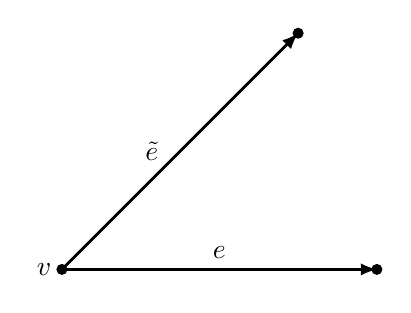
\begin{tikzpicture}[>=latex, line width=1pt, scale=1]

% vertex coords
\coordinate (V1) at (-2,0);
\coordinate (V2) at (2,0);
\coordinate (V3) at (1,3);


%points
\fill(V1) circle(2pt);
\fill(V2) circle(2pt);
\fill(V3) circle(2pt);

%arrows
\draw[->]  (V1) node[left]{$v$} -- (V2) node [midway,above] {$e$};
\draw[->]  (V1) -- (V3) node [midway,left=4pt] {$\tilde{e}$};



\end{tikzpicture}
        \caption{Zwei zusammenhängende Kanten \( e \sim \tilde{e} \).}
        \label{fig:oneVertexTwoEdges}
      \end{minipage}
      \hfill
      \begin{minipage}[b]{0.45\textwidth}
        \center
        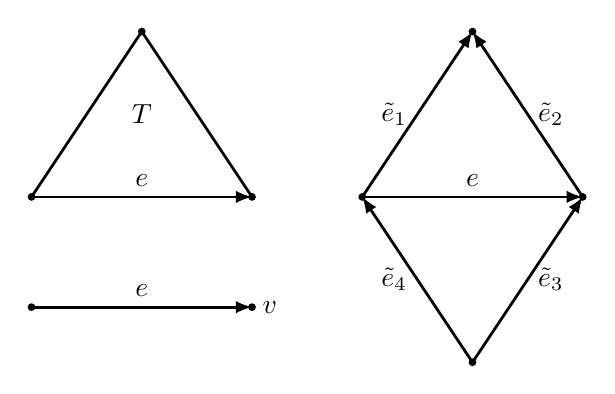
\begin{tikzpicture}[>=latex, line width=1pt, scale=0.7]

% vertex coords
\coordinate (V1) at (-2,0);
\coordinate (V2) at (2,0);
\coordinate (V3) at (0,3);
\coordinate (V4) at (0,-3);

%points
\fill(V1) circle(2pt);
\fill(V2) circle(2pt);
\fill(V3) circle(2pt);
\fill(V4) circle(2pt);

%arrows
\draw[->] (V1) -- (V2) node [midway,above] {$e$} ;
\draw[->] (V2) -- (V3) node [midway,right] {$\tilde{e}_{2}$};
\draw[->] (V1) -- (V3) node [midway,left] {$\tilde{e}_{1}$};
\draw[->] (V4) -- (V2) node [midway,right] {$\tilde{e}_{3}$};
\draw[->] (V4) -- (V1) node [midway,left] {$\tilde{e}_{4}$};



\coordinate (VV1) at (-8,0);
\coordinate (VV2) at (-4,0);
\coordinate (VV3) at (-6,3);

\fill(VV1) circle(2pt);
\fill(VV2) circle(2pt);
\fill(VV3) circle(2pt);

\draw[->] (VV1) -- (VV2) node [midway,above] {$e$} ;
\draw[] (VV2) -- (VV3) ;
\draw[] (VV1) -- (VV3) ;

\node at (-6,1.5) {$T$};



\coordinate (VVV1) at (-8,-2);
\coordinate (VVV2) at (-4,-2);

\fill(VVV1) circle(2pt);
\fill(VVV2) circle(2pt);

\draw[->] (VVV1) -- (VVV2) node [midway,above] {$e$} ;

\node[right] at (VVV2) {$v$};


\end{tikzpicture}

        \caption{Beispiel eines Kantenskeletts in der immer \( s_{e,\cdot} = +1\) gilt.}
        \label{fig:correctEdgeOrientation}
      \end{minipage}
    \end{figure}
    

  \subsubsection{Diskreter Hodge-Operator \( \circledast \)}
    Anders als in der DEC-Diskretisierung in \cite{Nestler2016} werden wir hier keine Hodge-duale Gleichung für die vektorwertige Identität \eqref{eq:NS1DisTime}
    zur Determinierung der Hodge-dualen Lösung \( *\Ub \) aufstellen.
    In Experimenten hat sich gezeigt, dass dieses Vorgehen zu einem instabilen Verfahren führt.
    Stattdessen werden wir \( *\Ub \) in jedem Zeitschritt direkt approximieren.

    
    Aus dem Beispiel \eqref{eq:hodgeApproxTwoEdges} wissen wir schon wie wir den Hodge-Operator bzgl. zwei Kanten approximieren können.
    Nun wollen wir aber keine einzelne zusätzliche Kante Vorrang gewähren und alle Kanten \( \tilde{e}\facesim e \) 
    wie in \autoref{fig:correctEdgeOrientation} mit einbeziehen.
    Also mitteln\footnote{\ingo{Obwohl das mitteln von Approximation unbekannter Freiheitsgrade im Allgemeinen keine gute Idee ist, aber hier klappt es.
                                Womöglich ein Hinweis darauf, dass eine Herleitung ohne Mittelung existiert, die auf das gleiche Ergebnis führt.}} 
    wir die Approximation \eqref{eq:hodgeApproxTwoEdges} über all diese Kanten und erhalten
    \begin{align}
      \left( *\U \right)(e) \approx \circledast \U (e)
            &:= \frac{1}{4}\sum_{\tilde{e}\facesim e}
                          \frac{s_{e\tilde{e}}}{\sqrt{\left| e \right|^{2}\left| \tilde{e} \right|^{2} 
                                                        - \left( \vect{e}\cdot\tilde{\vect{e}}\right)^{2}}}
                             \left( \left( \vect{e}\cdot\tilde{\vect{e}} \right) \U(e) 
                                   -\left| e \right|^{2}\U(\tilde{e}) \right) \formPeriod
    \end{align}
    Für andere Hodge-Operator-Approximationen siehe \cite{Mohamed2016}.

  \subsubsection{Diskreter Rot-rot-Laplace \( \lrr \)}
    Der Rot-rot-Laplace kann über \( (\lrr\U)(e) = \star\exd\star\exd\U(e) \) direkt nach dem beschrieben Vorgehen in \cite{Hirani2003} hergeleitet werden.
    In \cite{Nestler2016} ist er explizit aufgeführt mit 
    \begin{align} \label{eq:rotrotlaplace}
      (\lrr\U)(e) \approx \lrr\U(e)
          &:= -\frac{\left| e \right|}{\left| \star e \right|} \sum_{\face\succ e} \frac{s_{\face,e}}{\left| \face \right|}
                                \sum_{\tilde{e}\prec \face} s_{\face,\tilde{e}} \U(\tilde{e})
    \end{align}
    mit
    \begin{align}
      s_{\face,e} &:=
        \begin{cases}
          +1 & \text{if } e\prec \face \text{ and \( \face \) is on left side of \( e \)} \\
          -1 & \text{if } e\prec \face \text{ and \( \face \) is on right side of \( e \)} \\
           0 & e \nprec \face\formPeriod
        \end{cases}
    \end{align}

  \subsubsection{Diskrete äußere Ableitung \( \exd \)}
    Stokes-Theorem: \( (\exd q)(e) = \exd q (e) := q(v_{2}) - q(v_{1}) \) für \( e=\left[ v_{1}, v_{2} \right] \).


   
  \subsubsection{Diskreter rot-Operator auf Kantenmittelpunkt}
    Allgemein lässt sich die Rotation einer vektorwertigen Größe in einem Gebiet \( A \) als (counterclockwise) Integral entlang des Randes von \(A\)  berechnen.
    Formal schreiben wir für \( A = \sum_{\face\succ e}|\face| \)
    \begin{align}
      (\rot\Ub)(c(e)) = (*\exd\Ub)(c(e))
                     \approx  \frac{1}{\sum_{\face\succ e}|\face|}\sum_{\face\succ e}(\exd\Ub)(\face)
                     &= \frac{1}{\sum_{\face\succ e}|\face|}\sum_{\face\succ e}\sum_{\tilde{e}\prec\face}s_{\tilde{e}\face}\Ub(\tilde{e})\\
                     &= \frac{1}{\sum_{\face\succ e}|\face|}\sum_{\tilde{e}\facesim e} s_{\ldots} \Ub(\tilde{e})
    \end{align}
    mit Vorzeichen \( s_{\ldots} \) so gewählt, dass die Orientierung der Kanten \( \tilde{e} \) die der geerbten Orientierung der Fläche entsprechen.

    Somit können wir nun auch Ausdrücke der Art
    \begin{align}
      ((*\tilde{\Ub})\rot\Ub)(e) \approx \frac{(*\tilde{\Ub})(e)}{\sum_{\face\succ e}|\face|}\sum_{\tilde{e}\facesim e} s_{\ldots} \Ub(\tilde{e})
                        =: (*\tilde{\Ub})(e) \rot(\Ub)(e)
    \end{align}
    approximieren.

  \subsubsection{Diskreter Divergenz-Operator}
    Für Divergenz einer 1-Form an einer Ecke \( v \) siehe \cite{Hirani2003,DiplomIngo2014}.
    Für \( \tilde{\Ub} \) ergibt sich
    \begin{align}
      (\div\tilde{\Ub})(v) = (*\exd * \tilde{\Ub})(v) \approx \frac{1}{|\star v|}\sum_{\tilde{e}\succ v}s_{\ldots}\frac{|\star \tilde{e}|}{|\tilde{e}|}\tilde{\Ub}(\tilde{e})\formPeriod
    \end{align}
    wobei die Vorzeichen \( s_{\ldots} \) so gewählt werden, dass sie positiv sind, wenn die Kanten \( \tilde{e} \) von der Ecke \( v \) weg zeigen.

    Wenn wir die Divergenz einer bekannten Vektorgröße an einer Kante brauchen, so mitteln wir sie über beide Eckpunkte.
    So können wir auch den Term
    \begin{align}
      ((\div\tilde{\Ub})(*\Ub))(e) 
        &\approx \frac{1}{2}\left( \sum_{v\prec e} \frac{1}{|\star v|}\sum_{\tilde{e}\succ v}s_{\ldots}\frac{|\star \tilde{e}|}{|\tilde{e}|}\tilde{\Ub}(\tilde{e}) \right)
            (*\Ub)(e)
        =: \div(\tilde{\Ub})(e)(*\Ub)(e)
    \end{align}
    approximieren.

  \subsubsection{Diskretes inneres Produkt}
    Wie wir in \cite{Nestler2016} schon gesehen haben, können wir das innere Produkt am Kantenmittelpunkt \( c(e) \) durch
    \begin{align}
      \left\langle \tilde{\Ub} , \Ub \right\rangle(c(e))
          &\approx \frac{1}{\left| e \right|^{2}}\left( \tilde{\Ub}(e) \Ub(e) + \left( *\tilde{\Ub} \right)(e) \left( *\Ub \right)(e) \right)
    \end{align}
    approximieren.
    Um nun das innere Produkt auf einer Ecke auszuwerten nutzen wir eine Zerlegung der Voronoizelle zu
    \begin{align}
      \star v &= \sum_{e\succ v} A_{ve} \\
      \text{mit } \left|A_{ve}\right| &= \frac{\left| e \right|\left| \star e \right|}{4} \formPeriod
    \end{align}
    vgl. hierzu \autoref{fig:VCellDecomp}.
    \begin{figure}[tbp]
      \centering
      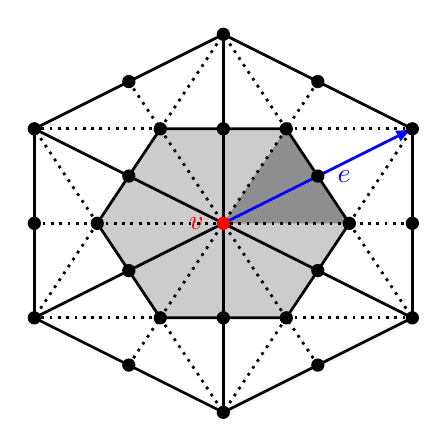
\begin{tikzpicture}[>=latex, line width=1pt, scale=1.2]
  % Coords
\coordinate (V0) at (2,0);
\coordinate (V1) at (2,2);
\coordinate (V2) at (0,1);
\coordinate (V3) at (4,1);
\coordinate (V4) at (4,-1);
\coordinate (V5) at (0,-1);
\coordinate (V6) at (2,-2);

%circumcenter
\coordinate (CC1) at (1.333,1);
\coordinate (CC0) at (2.666,1);
\coordinate (CC3) at (1.333,-1);
\coordinate (CC2) at (0.666,0);
\coordinate (CC4) at (2.666,-1);
\coordinate (CC5) at (3.333,0);

 
\coordinate (C01) at (2,1);
\coordinate (C02) at (1,0.5);
\coordinate (C03) at (3,0.5);
\coordinate (C05) at (1,-0.5);
\coordinate (C04) at (3,-0.5);
\coordinate (C06) at (2,-1);

\coordinate (C12) at (1,1.5);
\coordinate (C25) at (0,0);
\coordinate (C56) at (1,-1.5);
\coordinate (C46) at (3,-1.5);
\coordinate (C34) at (4,0);
\coordinate (C13) at (3,1.5);

\fill[black, opacity=0.2] (CC0) -- (CC1) -- (CC2) -- (CC3) -- (CC4) -- (CC5) -- (CC0);
\fill[black, opacity=0.3] (V0) -- (CC5) -- (CC0) -- (V0);
%\fill[opacity=0.4]  (V1) -- (V3) -- (V4) -- (V6) -- (V5) -- (V2);
  % Arrows\tilde{\sigma}
\draw[](V0) -- (V1);
\draw[](V1) --  (V2);
\draw[](V0) -- (V2);
\draw[](V1) --  (V3);
\draw[blue,->](V0) -- (V3);
\draw[](V0) -- (V4);
\draw[](V0) -- (V5);
\draw[](V5) --  (V2);
\draw[](V3) --  (V4);
\draw[](V4) -- (V6);
\draw[](V0) -- (V6);
\draw[](V6) -- (V5);
 
\draw (CC0) -- (CC1) -- (CC2) -- (CC3) -- (CC4) -- (CC5) -- (CC0);
\draw[dotted] (C12) -- (CC1);
\draw[dotted] (C25) -- (CC2);
\draw[dotted] (C56) -- (CC3);
\draw[dotted] (C46) -- (CC4);
\draw[dotted] (C34) -- (CC5);
\draw[dotted] (C13) -- (CC0);
\draw[dotted] (CC1) -- (CC4);
\draw[dotted] (CC2) -- (CC5);
\draw[dotted] (CC3) -- (CC0);

\draw[dotted] (CC1) -- (V1);
\draw[dotted] (CC2) -- (V2);
\draw[dotted] (CC3) -- (V5);
\draw[dotted] (CC4) -- (V6);
\draw[dotted] (CC5) -- (V4);
\draw[dotted] (CC0) -- (V3);

\draw[dotted] (CC1) -- (V2);
\draw[dotted] (CC2) -- (V5);
\draw[dotted] (CC3) -- (V6);
\draw[dotted] (CC4) -- (V4);
\draw[dotted] (CC5) -- (V3);
\draw[dotted] (CC0) -- (V1);

%\draw[blue,->] (CC5) -- (CC0); 

\fill[red] (V0) node[left] {\(v\ \)} circle (2pt);
\fill (V1) circle (2pt);
\fill (V2) circle (2pt);
\fill (V3) circle (2pt);
\fill (V4) circle (2pt);
\fill (V5)circle (2pt);
\fill (V6)circle (2pt);

\fill (CC0) circle (2pt);
\fill (CC1) circle (2pt);
\fill (CC2) circle (2pt);
\fill (CC3) circle (2pt);
\fill (CC4) circle (2pt);
\fill (CC5) circle (2pt);



\fill (C01) circle (2pt);
\fill (C02) circle (2pt);
\fill (C03) node[right, blue] {\(\ e\)}circle (2pt);
\fill (C05) circle (2pt);
\fill (C04) circle (2pt);
\fill (C06) circle (2pt);
 

\fill (C12) circle (2pt);
\fill (C25) circle (2pt);
\fill (C56) circle (2pt);
\fill (C46) circle (2pt);
\fill (C34) circle (2pt);
\fill (C13) circle (2pt);


\end{tikzpicture}


      \caption{Umkreismittelpunktsunterteilung. Die Voronoizelle \( \star v \) ist hellgrau hervor gehoben und deren Anteil \( A_{ve} \) dunkelgrau.}
      \label{fig:VCellDecomp}
    \end{figure}
    Somit erhalten wir mit konstanter Approximation des Flächenintegrals und formalen diskreten Kalkül
    \begin{align}
      \left\langle \tilde{\Ub} , \Ub \right\rangle(v)
          &\approx \frac{1}{\left| \star v \right|}\left( *\left\langle \tilde{\Ub} , \Ub \right\rangle  \right)(\star v) 
           = \frac{1}{\left| \star v \right|}\sum_{e\succ v}\left( *\left\langle \tilde{\Ub} , \Ub \right\rangle  \right)(A_{ve}) \\
          &\approx\frac{1}{\left| \star v \right|}\sum_{e\succ v} \frac{\left| e \right|\left| \star e \right|}{4}  \left\langle \tilde{\Ub} , \Ub \right\rangle(c(e)) \\
          &\approx\frac{1}{4\left| \star v \right|}\sum_{e\succ v} \frac{\left| \star e \right|}{\left| e \right|} \left( \tilde{\Ub}(e) \Ub(e) + \left( *\tilde{\Ub} \right)(e) \left( *\Ub \right)(e) \right)
           =: \textup{i}_{\tilde{\Ub}}\Ub(v)\formPeriod
    \end{align}
    Die innere Summe zerlegen wir nun in seinen primären und dualen Anteil, so dass für
    \begin{align}
      \jup_{\tilde{\Ub}}\Ub(v) := \frac{1}{4\left| \star v \right|}\sum_{e\succ v} \frac{\left| \star e \right|}{\left| e \right|} \tilde{\Ub}(e) \Ub(e)
    \end{align}
    \( \textup{i}_{\tilde{\Ub}}\Ub(v) =  \jup_{\tilde{\Ub}}\Ub(v) + \jup_{*\tilde{\Ub}}(*\Ub)(v)\) gilt.

\subsection{Diskretes lineares System}
  Zusammenfassend ist nun für \( k=0,1,\ldots \) folgendes lineares Gleichungssystem 
  für \\\( \Ub_{k+1}, (*\Ub)_{k+1} \in \Lambda^{1}_{h}(\SC)\) und \( q_{k+1} , p_{k+1} \in \Lambda^{0}_{h}(\SC) \) zulösen:
  \begin{align}
    \circledast\Ub_{k+1} - (*\Ub)_{k+1} &= 0 \label{eq:NS0Dis}\\
    \frac{1}{\tau_{k}}\Ub_{k+1} - \nu\left( \lrr\Ub_{k+1} + 2\gauss\Ub_{k+1} \right) + \exd q_{k+1}
        &+ (*\Ub)_{k}\rot\Ub_{k+1} - \div((*\Ub)_{k})(*\Ub)_{k+1} \notag\\
              &= \frac{1}{\tau_{k}}\Ub_{k} + (*\Ub)_{k}\rot\Ub_{k} \label{eq:NS1Dis}\\
     \jup_{\Ub_{k}}\Ub_{k+1} + \jup_{(*\Ub)_{k}}(*\Ub)_{k+1} + \P_{k+1} - q_{k+1} 
          &= \frac{1}{2}\left( \jup_{\Ub_{k}}\Ub_{k} + \jup_{(*\Ub)_{k}}(*\Ub)_{k} \right) \label{eq:NS2Dis}\\
    \div\Ub_{k+1} &= 0 \label{eq:NS3Dis}
  \end{align}
  für alle \( e\in\Es \) in Gleichungen \eqref{eq:NS0Dis}, \eqref{eq:NS1Dis}  und alle \( v\in\Vs \) in Gleichungen \eqref{eq:NS2Dis}, \eqref{eq:NS3Dis}
  und Startlösung \(  \Ub_{0}, (*\Ub)_{0}, q_{0}\) und \( p_{0}\).
  Die Argumente \( e \) bzw. \( v \) wurden hierbei für eine bessere Lesbarkeit weggelassen.
  Bei einer geeigneten Assemblierung führt dieses System zu einer dünnbesetzten Systemmatrix 
  \( M_{k+1}\in\R^{2(|\Es| + |\Vs|)\times 2(|\Es| + |\Vs|)} \) und Rechte-Seite-Vektor 
  \( r_{k}\in\R^{2(|\Es| + |\Vs|)} \).
  Um den Druck zu determinieren ersetzen wir eine Zeile in \( M_{k+1} \) und \( r_{k} \) so, 
  dass dieses gerade \( p_{k+1}(v_{0}) = 0 \) am Knoten \( v_{0}\in\Vs \) erfüllt.
  Das Gleichungssystem wird mit \( \texttt{umfpack} \) gelöst.

\subsection{DEC-Diskretisierung im Staggered-Grid (Arakawa C-grid)}
  
    \begin{figure}[tbp]
      \centering
      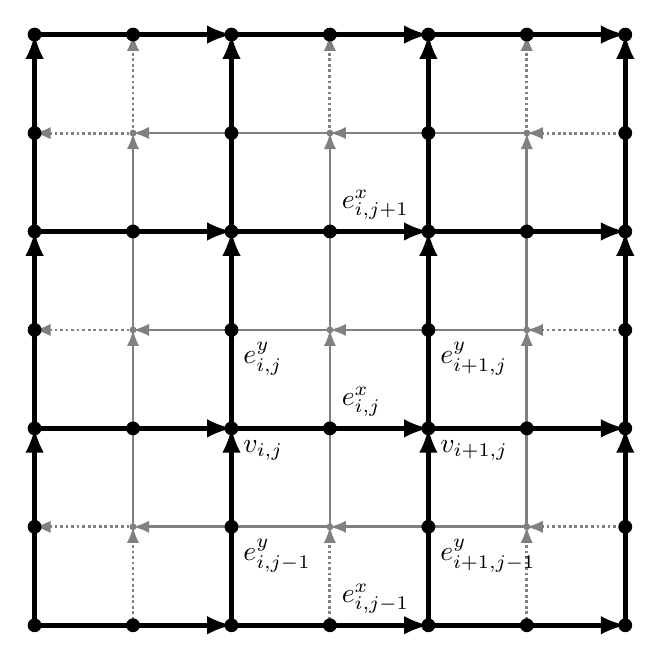
\begin{tikzpicture}[>=latex, line width=2pt, scale=2.5]
\usetikzlibrary{calc}

\edef\n{3}

\pgfmathparse{\n-1}
\edef\nmone{\pgfmathresult}

\pgfmathparse{\n-2}
\edef\nmtwo{\pgfmathresult}

%all the gray (dual) stuff
\begin{scope}[gray,  line width=1pt]
%dual vertices
\foreach \x in {0,...,\nmone} {
	\foreach \y in {0,...,\nmone} {
		\coordinate (V) at (\x+0.5,\y+0.5);
		\fill (V) circle(0.5pt);
	}
}

%dual x-edges
\foreach \x in {0,...,\nmtwo} {
	\foreach \y in {0,...,\nmone} {
		\coordinate (V1) at (\x+0.5,\y+0.5);
		\coordinate (V2) at (\x+1.5,\y+0.5); 
		\draw[<-] (V1) -- (V2);
	}
}

%dual y-edges
\foreach \x in {0,...,\nmone} {
	\foreach \y in {0,...,\nmtwo} {
		\coordinate (V1) at (\x+0.5,\y+0.5);
		\coordinate (V2) at (\x+0.5,\y+1.5); 
		\draw[->] (V1) -- (V2);
	}
}

%all remaining (half) dual edges on the boundaries 
\foreach \xy in {0,...,\nmone} {
	\draw[->,densely dotted] (\xy+0.5, 0) --  (\xy+0.5, 0.5); 
	\draw[->,densely dotted] (\xy+0.5, \n-0.5) --  (\xy+0.5, \n);
	\draw[<-,densely dotted] (0,\xy+0.5) -- (0.5,\xy+0.5);
	\draw[<-,densely dotted] (\n-0.5,\xy+0.5) -- (\n,\xy+0.5);
}
\end{scope}

%primal vertices
\foreach \x in {0,...,\n} {
	\foreach \y in {0,...,\n} {
		\coordinate (V) at (\x,\y);
		\fill (V) circle(1pt);
	}
}

%primal x-edges
\foreach \x in {0,...,\nmone} {
	\foreach \y in {0,...,\n} {
		\coordinate (V1) at (\x,\y);
		\coordinate (V2) at (\x+1,\y); 
		\draw[->] (V1) -- (V2);
	}
}

%primal y-edges
\foreach \x in {0,...,\n} {
	\foreach \y in {0,...,\nmone} {
		\coordinate (V1) at (\x,\y);
		\coordinate (V2) at (\x,\y+1); 
		\draw[->] (V1) -- (V2);
	}
}

%primal edge circumcenters
\foreach \xy in {0,...,\n} {
	\foreach \yx in {0,...,\nmone} {
		\coordinate (VX) at (\yx+0.5,\xy);
		\coordinate (VY) at (\xy,\yx+0.5);
		\fill (VX) circle(1pt);
		\fill (VY) circle(1pt);
	}
}

%nodes
\node[below right] at (1,1) {$v_{i,j}$};
\node[below right] at (2,1) {$v_{i+1,j}$};

\node[above right] at (1.5,1) {$e^x_{i,j}$};
\node[above right] at (1.5,0) {$e^x_{i,j-1}$};
\node[above right] at (1.5,2) {$e^x_{i,j+1}$};

\node[below right] at (1,1.5) {$e^y_{i,j}$};
\node[below right] at (2,1.5) {$e^y_{i+1,j}$};
\node[below right] at (1,0.5) {$e^y_{i,j-1}$};
\node[below right] at (2,0.5) {$e^y_{i+1,j-1}$};



\end{tikzpicture}
      \caption{Staggered-Grid (Arakawa C-grid) mit dualem Gitter und Orientierungen.
               Vektorkomponenten, wie das Geschwindigkeitsfeld, in \( x \)- bzw. \( y \)-Richtung sind auf den Kantenmittelpunkten 
               der horizentalen bzw. vertikalen Kanten \( e^{x} \) bzw. \( e^{y} \) definiert. 
               Skalare, wie der Druck, sind auf den Ecken \( v \) definiert.}
      \label{fig:staggeredGrid}
    \end{figure}

Wir wollen uns nun anschauen, welche DEC-Diskretisierung sich auf einen uniformen flachen Gitter ergibt.
In diesem Fall können wir einfachheitshalber statt Dreiecke auch Quadrate nutzen,
da die (signierten) Höhen im Quadrat sich in einem eindeutigen Punkt treffen und somit die dualen Kanten klar definiert sind.
Das sich ergebene Gitter ist ein Staggered-Grid (Arakawa C-grid, siehe \cite{Arakawa1977}) und in \autoref{fig:staggeredGrid}
dargestellt. 

Identifizieren wir Vektorkomponenten \( u^{x} \) und \( u^{y} \) in den Kantenmittelpunkten als Integralmittel der diskreten 1-Form,
so ergibt sich mit einer Kantenlänge \( h \) und den Bezeichnern in \autoref{fig:staggeredGrid}
\begin{align}
  u^{x}_{ij} &:= u^{x}(c(e^{x}_{i,j}))
                = \frac{1}{h} \U_{h}(e^{x}_{i,j}) \\
  u^{y}_{ij} &:= u^{y}(c(e^{y}_{i,j}))
                = \frac{1}{h} \U_{h}(e^{y}_{i,j}) 
\end{align}
und für skalare Größen \( q \)
\begin{align}
  q_{i,j} := q(v_{i,j}) = q_{h}(v_{i,j}) \formPeriod
\end{align}
\ingo{Die Auswertungsklammern sind missdeutig. Es ist zu überlegen, ob es nicht besser wäre eckige Klammern zur Auswertung von diskreten Formen zu verwenden, d.h. z.B. \( \U_{h}[e] \).}
Es sei hier darauf hingewiesen, dass wir uns im flachen zweidimensionalen Raum bewegen mit allen Konsequenzen, wie z.B. \( \gauss = 0 \).
Wir wollen im Folgendem darauf nicht mehr explizit eingehen.

  \subsubsection{Laplace-Operatoren}
    \begin{figure}[tbp]
      \centering
      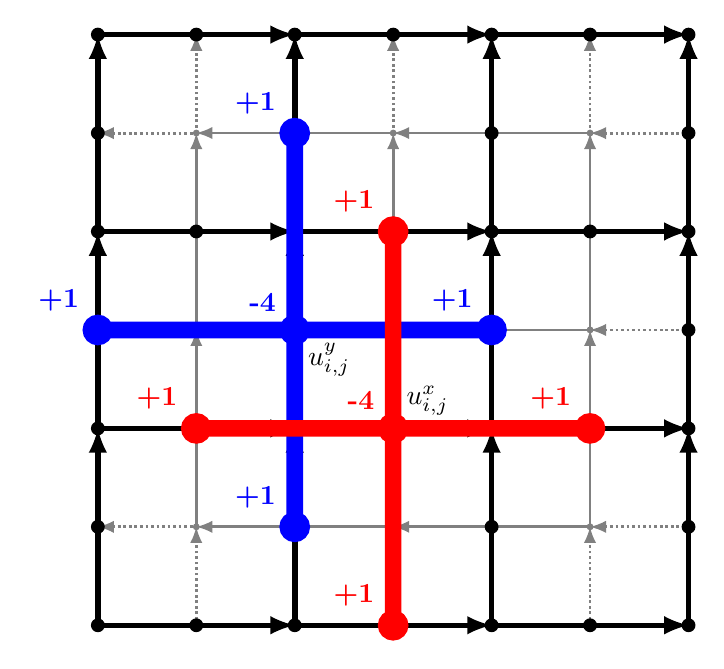
\begin{tikzpicture}[>=latex, line width=2pt, scale=2.5]
\usetikzlibrary{calc}

\bf
\edef\n{3}

\pgfmathparse{\n-1}
\edef\nmone{\pgfmathresult}

\pgfmathparse{\n-2}
\edef\nmtwo{\pgfmathresult}

%all the gray (dual) stuff
\begin{scope}[gray,  line width=1pt]
%dual vertices
\foreach \x in {0,...,\nmone} {
	\foreach \y in {0,...,\nmone} {
		\coordinate (V) at (\x+0.5,\y+0.5);
		\fill (V) circle(0.5pt);
	}
}

%dual x-edges
\foreach \x in {0,...,\nmtwo} {
	\foreach \y in {0,...,\nmone} {
		\coordinate (V1) at (\x+0.5,\y+0.5);
		\coordinate (V2) at (\x+1.5,\y+0.5); 
		\draw[<-] (V1) -- (V2);
	}
}

%dual y-edges
\foreach \x in {0,...,\nmone} {
	\foreach \y in {0,...,\nmtwo} {
		\coordinate (V1) at (\x+0.5,\y+0.5);
		\coordinate (V2) at (\x+0.5,\y+1.5); 
		\draw[->] (V1) -- (V2);
	}
}

%all remaining (half) dual edges on the boundaries 
\foreach \xy in {0,...,\nmone} {
	\draw[->,densely dotted] (\xy+0.5, 0) --  (\xy+0.5, 0.5); 
	\draw[->,densely dotted] (\xy+0.5, \n-0.5) --  (\xy+0.5, \n);
	\draw[<-,densely dotted] (0,\xy+0.5) -- (0.5,\xy+0.5);
	\draw[<-,densely dotted] (\n-0.5,\xy+0.5) -- (\n,\xy+0.5);
}
\end{scope}

%primal vertices
\foreach \x in {0,...,\n} {
	\foreach \y in {0,...,\n} {
		\coordinate (V) at (\x,\y);
		\fill (V) circle(1pt);
	}
}

%primal x-edges
\foreach \x in {0,...,\nmone} {
	\foreach \y in {0,...,\n} {
		\coordinate (V1) at (\x,\y);
		\coordinate (V2) at (\x+1,\y); 
		\draw[->] (V1) -- (V2);
	}
}

%primal y-edges
\foreach \x in {0,...,\n} {
	\foreach \y in {0,...,\nmone} {
		\coordinate (V1) at (\x,\y);
		\coordinate (V2) at (\x,\y+1); 
		\draw[->] (V1) -- (V2);
	}
}

%primal edge circumcenters
\foreach \xy in {0,...,\n} {
	\foreach \yx in {0,...,\nmone} {
		\coordinate (VX) at (\yx+0.5,\xy);
		\coordinate (VY) at (\xy,\yx+0.5);
		\fill (VX) circle(1pt);
		\fill (VY) circle(1pt);
	}
}

%schemata
\draw[blue, line width=6pt] (0,1.5) circle(1pt) node[above left]{+1} -- (1,1.5) circle(1pt) node[above left]{-4}  -- (2,1.5) circle(1pt)node[above left]{+1};
\draw[blue, line width=6pt] (1,0.5) circle(1pt) node[above left]{+1} -- (1,2.5) circle(1pt)node[above left]{+1};

\draw[red, line width=6pt] (0.5,1) circle(1pt) node[above left]{+1} -- (1.5,1) circle(1pt) node[above left]{-4}  -- (2.5,1) circle(1pt)node[above left]{+1};
\draw[red, line width=6pt] (1.5,0) circle(1pt) node[above left]{+1} -- (1.5,2) circle(1pt)node[above left]{+1};

%nodes
%\node[below right] at (1,1) {$v_{i,j}$};
%\node[below right] at (2,1) {$v_{i+1,j}$};

\node[above right] at (1.5,1) {$u^x_{i,j}$};
%\node[above right] at (1.5,0) {$e^x_{i,j-1}$};
%\node[above right] at (1.5,2) {$e^x_{i,j+1}$};

\node[below right] at (1,1.5) {$u^y_{i,j}$};
%\node[below right] at (2,1.5) {$e^y_{i+1,j}$};
%\node[below right] at (1,0.5) {$e^y_{i,j-1}$};
%\node[below right] at (2,0.5) {$e^y_{i+1,j-1}$};



\end{tikzpicture}

      \caption{Schemata für \( \Delta u^{x} \) (rot) bzw. \( \Delta u^{y} \) (blau) auf dem Staggered-Grid.
                Die DEC-Diskretisierung liefert hier den bekannten 5-Punkt-Stempel.}
      \label{fig:deRhamStaggeredGrid}
    \end{figure}

    In Finite-Differenzen-Diskretisierungen der Navier-Stokes-Gleichungen in einer Ebene wird für gewöhnlich der ''volle'' Laplace-Operator
    \begin{align}
      \Delta = -\ldr = \lrr + \lgd
    \end{align}
    diskretisiert (siehe z.B. \cite{Armfield1991}).
    \( \lgd = \nabla\div \) ist der Grad-div-Laplace-Operator, der wegen der Divergenzfreiheit null ergibt.
    Das bedeutet, dass im Kontinuierlichem \( \Delta \) und \( \lrr \) eingeschränkt auf divergenzfreie Vektorfelder das gleiche sind.
    Jedoch ist die Diskretisierung eine andere.
    Für \( \Delta = -\ldr \) ergeben sich mit der DEC-Diskretisierung an \( c(e^{x}_{i,j}) \) bzw. \(c(e^{y}_{i,j})\) in \cite{Nestler2016} folgende
    Schemata
    \begin{align}
      (\Delta u)^{\{x,y\}}_{i,j} &= \frac{1}{h}\ldr\U_{h}(e^{\{x,y\}}_{i,j})
                                \overset{DEC}{=} \frac{1}{h}\U_{h}\left( e^{\{x,y\}}_{i+1,j} +  e^{\{x,y\}}_{i-1,j} 
                                                      +e^{\{x,y\}}_{i,j+1} +  e^{\{x,y\}}_{i,j-1}
                                                      -4e^{\{x,y\}}_{i,j}\right) \\
                      &= \frac{1}{h^{2}}\left( u^{\{x,y\}}_{i+1,j} +  u^{\{x,y\}}_{i-1,j} 
                                                      +u^{\{x,y\}}_{i,j+1} +  u^{\{x,y\}}_{i,j-1}
                                                      -4u^{\{x,y\}}_{i,j} \right) \formPeriod
    \end{align}
    Das ist der bekannte 5-Punkt-Stempel (vgl. \autoref{fig:deRhamStaggeredGrid}) in beiden Koordinatenrichtungen mit Konsistenzordnung \( \landau(h^{2}) \).
    \begin{figure}[tbp]
      \centering
      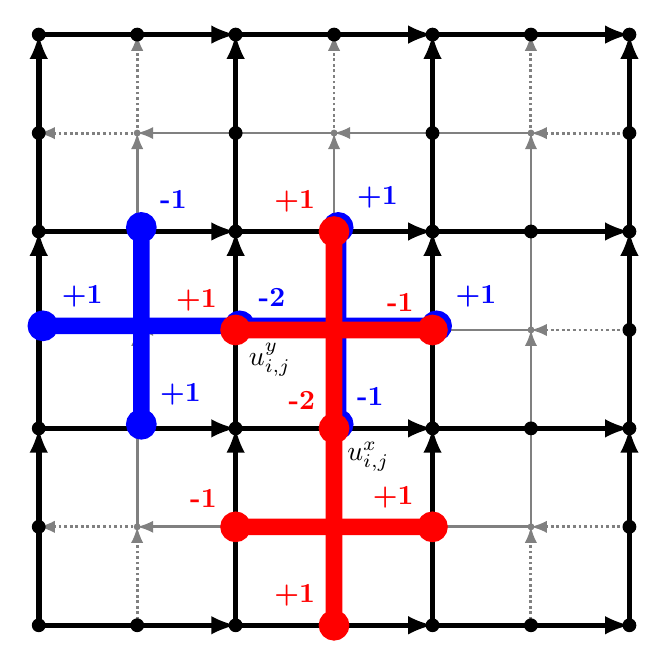
\begin{tikzpicture}[>=latex, line width=2pt, scale=2.5]
\usetikzlibrary{calc}
\bf
\edef\n{3}

\pgfmathparse{\n-1}
\edef\nmone{\pgfmathresult}

\pgfmathparse{\n-2}
\edef\nmtwo{\pgfmathresult}

%all the gray (dual) stuff
\begin{scope}[gray,  line width=1pt]
%dual vertices
\foreach \x in {0,...,\nmone} {
	\foreach \y in {0,...,\nmone} {
		\coordinate (V) at (\x+0.5,\y+0.5);
		\fill (V) circle(0.5pt);
	}
}

%dual x-edges
\foreach \x in {0,...,\nmtwo} {
	\foreach \y in {0,...,\nmone} {
		\coordinate (V1) at (\x+0.5,\y+0.5);
		\coordinate (V2) at (\x+1.5,\y+0.5); 
		\draw[<-] (V1) -- (V2);
	}
}

%dual y-edges
\foreach \x in {0,...,\nmone} {
	\foreach \y in {0,...,\nmtwo} {
		\coordinate (V1) at (\x+0.5,\y+0.5);
		\coordinate (V2) at (\x+0.5,\y+1.5); 
		\draw[->] (V1) -- (V2);
	}
}

%all remaining (half) dual edges on the boundaries 
\foreach \xy in {0,...,\nmone} {
	\draw[->,densely dotted] (\xy+0.5, 0) --  (\xy+0.5, 0.5); 
	\draw[->,densely dotted] (\xy+0.5, \n-0.5) --  (\xy+0.5, \n);
	\draw[<-,densely dotted] (0,\xy+0.5) -- (0.5,\xy+0.5);
	\draw[<-,densely dotted] (\n-0.5,\xy+0.5) -- (\n,\xy+0.5);
}
\end{scope}

%primal vertices
\foreach \x in {0,...,\n} {
	\foreach \y in {0,...,\n} {
		\coordinate (V) at (\x,\y);
		\fill (V) circle(1pt);
	}
}

%primal x-edges
\foreach \x in {0,...,\nmone} {
	\foreach \y in {0,...,\n} {
		\coordinate (V1) at (\x,\y);
		\coordinate (V2) at (\x+1,\y); 
		\draw[->] (V1) -- (V2);
	}
}

%primal y-edges
\foreach \x in {0,...,\n} {
	\foreach \y in {0,...,\nmone} {
		\coordinate (V1) at (\x,\y);
		\coordinate (V2) at (\x,\y+1); 
		\draw[->] (V1) -- (V2);
	}
}

%primal edge circumcenters
\foreach \xy in {0,...,\n} {
	\foreach \yx in {0,...,\nmone} {
		\coordinate (VX) at (\yx+0.5,\xy);
		\coordinate (VY) at (\xy,\yx+0.5);
		\fill (VX) circle(1pt);
		\fill (VY) circle(1pt);
	}
}

%schemata
\edef\sh{0.6pt}
\draw[blue, yshift=\sh, xshift=\sh, line width=6pt] (0,1.5) circle(1pt) node[above right]{+1} -- (1,1.5) circle(1pt) node[above right]{-2}  -- (2,1.5) circle(1pt)node[above right]{+1};
\draw[blue, yshift=\sh, xshift=\sh, line width=6pt] (0.5,1)circle(1pt) node[above right]{+1} -- (0.5,2) circle(1pt)node[above right]{-1};
\draw[blue, yshift=\sh, xshift=\sh, line width=6pt] (1.5,1)circle(1pt) node[above right]{-1} -- (1.5,2) circle(1pt)node[above right]{+1};

\draw[red, line width=6pt] (1.5,0) circle(1pt) node[above left]{+1} -- (1.5,1) circle(1pt) node[above left]{-2}  -- (1.5,2) circle(1pt)node[above left]{+1};
\draw[red, line width=6pt] (1,1.5) circle(1pt) node[above left]{+1} -- (2,1.5) circle(1pt)node[above left]{-1};
\draw[red, line width=6pt] (1,0.5) circle(1pt) node[above left]{-1} -- (2,0.5) circle(1pt)node[above left]{+1};



%nodes
%\node[below right] at (1,1) {$v_{i,j}$};
%\node[below right] at (2,1) {$v_{i+1,j}$};

\node[below right] at (1.5,1) {$u^x_{i,j}$};
%\node[above right] at (1.5,0) {$e^x_{i,j-1}$};
%\node[above right] at (1.5,2) {$e^x_{i,j+1}$};

\node[below right] at (1,1.5) {$u^y_{i,j}$};
%\node[below right] at (2,1.5) {$e^y_{i+1,j}$};
%\node[below right] at (1,0.5) {$e^y_{i,j-1}$};
%\node[below right] at (2,0.5) {$e^y_{i+1,j-1}$};



\end{tikzpicture}
      \caption{Schemata für \( \lrr u^{x} \) (rot) bzw. \( \lrr u^{y} \) (blau) auf dem Staggered-Grid.}
      \label{fig:rotrotStaggeredGrid}
    \end{figure}
    Für den Rot-rot-Laplace-Operator
    \begin{align}
      \left( \lrr u \right)^{x} &= \partial_{y}^{2}u^{x} - \partial_{x}\partial_{y}u^{y} \\
      \left( \lrr u \right)^{y} &= \partial_{x}^{2}u^{y} - \partial_{x}\partial_{y}u^{x}
    \end{align}
    ergibt sich mit der DEC-Diskretisierung \eqref{eq:rotrotlaplace} und obiges Integralmittel 
    \begin{align}
      (\lrr u)^{x}_{i,j} &= \frac{1}{h^{2}}\left( u^{x}_{i,j+1} +  u^{x}_{i,j-1} - 2u^{x}_{i,j}
                                                 +u^{y}_{i,j} - u^{y}_{i+1,j}
                                                 +u^{y}_{i+1,j-1} -u^{y}_{i,j-1} \right) \\
      (\lrr u)^{y}_{i,j} &= \frac{1}{h^{2}}\left( u^{y}_{i+1,j} +  u^{y}_{i-1,j} - 2u^{y}_{i,j}
                                                 -u^{x}_{i,j} + u^{x}_{i,j+1}
                                                 -u^{x}_{i-1,j+1} +u^{x}_{i-1,j} \right) \formComma
    \end{align}
    wie in \autoref{fig:rotrotStaggeredGrid}) dargestellt.
    Dieser eher unübliche Diefferenzen-Stempel hat ebenfalls eine Konsistenz von \( \landau(h^{2}) \),
    wie wir im Folgendem o.E.d.A\footnote{durch Vierteldrehung des Gitters gegen den Uhrzeigersinn} für die \( x \)-Richtung zeigen wollen.

    Die ersten drei Summanden stellen die bekannte Approximation
    \begin{align}
      \frac{1}{h^{2}}\left( u^{x}_{i,j+1} +  u^{x}_{i,j-1} - 2u^{x}_{i,j}\right)
          &= \left( \partial_{y}^{2}u^{x} \right)^{x}_{i,j} + \landau(h^{2})
    \end{align}
    am Kantenmittelpunkt \( c(e^{x}_{i,j}) \) dar.
    Für die übrigen vier Summanden werden wir zweimal Taylor-approximieren in die jeweiligen Koordinatenrichtungen.
    Zuerst entwickeln wir in \( \pm y \)-Richtung an den Ecken \( v_{i+k,j} \) für \( k\in\left\{ 0,1 \right\} \) zu
    \begin{align}
      u^{y}_{i+k,j-l} 
          = \left( u^{y} + (-1)^{l} \frac{h}{2}\partial_{y}u^{y} + \frac{h^{2}}{8}\partial_{y}^{2}u^{y} 
                    + (-1)^{l}\frac{h^{3}}{48}\partial_{y}^{3}u^{y} + \frac{h^{4}}{384}\partial_{y}^{4}u^{y}\right)_{i+k,j}
             +\landau(h^{5})
    \end{align}
    für \( l\in\left\{ 0,1 \right\} \).
    Entwickeln wir weiter in \( \pm x \)-Richtung am Kantenmittelpunkt \( c(e^{x}_{i,j}) \), so erhalten wir
    \begin{align}
      u^{y}_{i+k,j-l}
        = \Big( &u^{y} + (-1)^{k+1}\frac{h}{2}\partial_{x}u^{y} + \frac{h^{2}}{8}\partial_{x}^{2}u^{y} 
                    + (-1)^{k+1}\frac{h^{3}}{48}\partial_{x}^{3}u^{y} + \frac{h^{4}}{384}\partial_{x}^{4}u^{y}  \\
                 &+(-1)^{l} \frac{h}{2}\partial_{y}u^{y} + (-1)^{l+k+1} \frac{h^{2}}{4}\partial_{x}\partial_{y}u^{y}
                      +(-1)^{l} \frac{h^{3}}{16}\partial_{x}^{2}\partial_{y}u^{y} + (-1)^{l+k+1} \frac{h^{4}}{96}\partial_{x}^{3}\partial_{y}u^{y} \\
                 &+ \frac{h^{2}}{8}\partial_{y}^{2}u^{y} + (-1)^{k+1} \frac{h^{3}}{16}\partial_{x}\partial_{y}^{2}u^{y}
                      + \frac{h^{4}}{64}\partial_{x}^{2}\partial_{y}^{2}u^{y} \\
                 &+(-1)^{l}\frac{h^{3}}{48}\partial_{y}^{3}u^{y} + (-1)^{l+k+1} \frac{h^{4}}{96}\partial_{x}\partial_{y}^{3}u^{y} \\
                 &+ \frac{h^{4}}{384}\partial_{y}^{4}u^{y}\Big)^{x}_{i,j} + \landau(h^{5}) \formPeriod
    \end{align}
    Aufsummieren ergibt
    \begin{align}
      \frac{1}{h^{2}}\left( u^{y}_{i,j} - u^{y}_{i+1,j} + u^{y}_{i+1,j-1} -u^{y}_{i,j-1} \right)
          &= -\left( \partial_{x}\partial_{y}u^{y} 
              + \frac{h^{2}}{96}\partial_{x}\partial_{y}\left( \partial_{x}^{2}u^{y} + \partial_{y}^{2}u^{y} \right)\right)^{x}_{i,j}
              +\landau(h^{3}) \\
          &= -\left( \partial_{x}\partial_{y}u^{y} \right)^{x}_{i,j}  +\landau(h^{2})
    \end{align}
    und somit die Behauptung.

    

\section{Appendix}

\subsection{Approximation diskreter 1-Formen auf abstrakter Kante an gerader Kante} \label{sec:approxOneForm}

\( e \) Kante, 
\( \pi \) Projektion auf abstrakte Kante, also \( \pi(e)\subset\surf \), 
\( \lambda \) Laufvariable auf Kante,
\(h_{e}(\lambda)  \) Höhe von Kante \( e \) zu \( \pi(e) \) an stelle \( \lambda \),
\( \alpha_{\xi}(\lambda) \) Normalenanteil bzgl Kante \( e \), der von \( \hat{\alpha} \) kommt bei Paralleltransport,

\begin{align}\label{eq:approxOneForm}
  \int_{\pi(e)}\hat{\alpha} = \int_{e}\alpha - |e|\int_{e}h_{e}(\lambda)\alpha_{\xi}'(\lambda)d\lambda + \mathcal{O}(h^{2}_{e,\max}|e|)
\end{align}

Beweis später.


\bibliography{bibl}
\bibliographystyle{alpha}

\end{document}
